
\chapter{\label{cha:Benchmarks}Benchmarks}


\section{Overview}

The Crustal Deformation Modeling and Earthquake Source Physics Focus
Groups within the Southern California Earthquake Center and the Short-Term
Tectonics Working Group within CIG have developed a suite of benchmarks
to test the accuracy and performance of 3D numerical codes for quasi-static
crustal deformation and earthquake rupture dynamics. The benchmark
definitions for the quasi-static crustal deformation benchmarks are
posted on the CIG website at Short-Term Tectonics Benchmarks \url{geodynamics.org/cig/workinggroups/short/workarea/benchmarks/}
and the definitions for the earthquake rupture benchmarks are posted
on the SCEC website \url{scecdata.usc.edu/cvws/cgi-bin/cvws.cgi}.
This suite of benchmarks permits evaluating the relative performance
of different types of basis functions, quadrature schemes, and discretizations
for geophysical applications. The files needed to run the 3D benchmarks
are in the CIG GitHub Repository \url{https://github.com/geodynamics/pylith_benchmarks}.
In addition to evaluating the efficiency and accuracy of numerical
codes, the benchmarks also make good test problems, where users can
perform simulations based on actual geophysical problems. The benchmarks
are performed at various resolutions and using different element types.
By comparing the runtime and accuracy for different resolutions and
element types, users can evaluate which combination will be best for
their problems of interest.


\section{\label{sec:benchmarks:strikeslip}Strike-Slip Benchmark}

This benchmark problem computes the viscoelastic (Maxwell) relaxation
of stresses from a single, finite, strike-slip earthquake in 3D without
gravity.  Dirichlet boundary conditions equal to the analytical elastic
solution are imposed on the sides of a cube with sides of length 24
km. Anti-plane strain boundary conditions are imposed at y = 0, so
the solution is equivalent to that for a domain with a 48 km length
in the y direction. We can use the analytical solution of \cite{Okada:1992}
both to apply the boundary conditions and to compare against the numerically-computed
elastic solution.




\subsection{Problem Description}

Figure \ref{fig:benchmark:strikeslip:geometry} shows the geometry
of the strike-slip fault (red surface) embedded in the cube consisting
of an elastic material (yellow block) over a Maxwell viscoelastic
material (blue block). 
\begin{description}
\item [{Domain}] The domain spans the region
\begin{gather*}
0\leq x\leq24\ km,\\
0\leq y\leq24\ km,\\
-24\ km\leq z\leq0.
\end{gather*}
The top (elastic) layer occupies the region $-12\ km\ \leq z\leq0$
and the bottom (viscoelastic) layer occupies the region $-24\ km\ \leq z\leq-12\ km$.
\item [{Material~properties}] The material is a Poisson solid with a shear
modulus of 30 GPa. The domain is modeled using an elastic isotropic
material for the top layer and a Maxwell viscoelastic material for
the bottom layer. The bottom layer has a viscosity of 1.0e+18 Pa-s.
\item [{Fault}] The fault is a vertical, right-lateral strike-slip fault.
The strike is parallel to the y-direction at the center of the model:
\begin{gather*}
x=12\ km,\\
0\leq y\leq16\ km,\\
-16\ km\leq z\leq0.
\end{gather*}
Uniform slip of 1 m is applied over the region $0\leq y\leq12\ km$
and $-12\ km\leq z\leq0$ with a linear taper to 0 at y = 16 km and
z = -16 km. The tapered region is the light red portion of the fault
surface in Figure \ref{fig:benchmark:strikeslip:geometry}. In the
region where the two tapers overlap, each slip value is the minimum
of the two tapers (so that the taper remains linear).
\item [{Boundary~conditions}] Bottom and side displacements are set to
the elastic analytical solution, and the top of the model is a free
surface. There are two exceptions to these applied boundary conditions.
The first is on the y=0 plane, where y-displacements are left free
to preserve symmetry, and the x- and z-displacements are set to zero.
The second is along the line segment between (12, 0, -24) and (12,
24, -24), where the analytical solution blows up in some cases. Along
this line segment, all three displacement components are left free.
\item [{Discretization}] The model is discretized with nominal spatial
resolutions of 1000 m, 500 m, and 250 m.
\item [{Basis~functions}] We use trilinear hexahedral cells and linear
tetrahedral cells.
\item [{Solution}] We compute the error in the elastic solution and compare
the solution over the domain after 0, 1, 5, and 10 years.
\end{description}
\noindent \begin{center}
\begin{figure}[H]
\begin{centering}
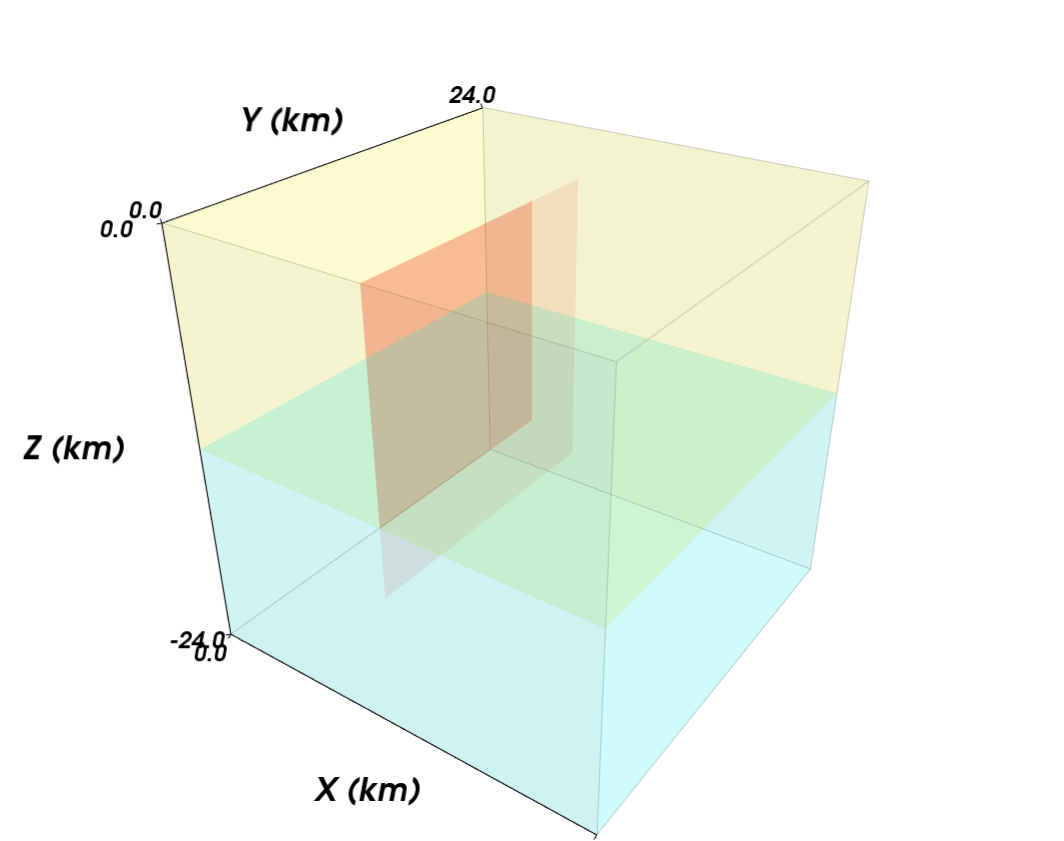
\includegraphics[scale=0.33]{benchmarks/strikeslip/figs/geometry}
\par\end{centering}

\caption{Geometry of strike-slip benchmark problem.\label{fig:benchmark:strikeslip:geometry}}
\end{figure}

\par\end{center}


\subsection{Running the Benchmark}

After checking out the benchmark files from the CIG SVN repository,
change to the \texttt{quasistatic/strikeslip} directory. Decompress
the gzipped files in the meshes and parameters directories,
\begin{lyxcode}
gunzip~meshes/{*}.gz~parameters/{*}.gz
\end{lyxcode}
Change to the parameters directory. Each benchmark uses three \texttt{.cfg}
files: \texttt{pylithapp.cfg}, a mesher related file (\texttt{strikeslip\_cubit.cfg}
or \texttt{strikeslip\_lagrit.cfg}), and a resolution and cell related
file (e.g., \texttt{strikeslip\_hex8\_1000m.cfg}). A few examples
of running the benchmarks (elastic solution only) are
\begin{lyxcode}
pylith~strikeslip\_cubit.cfg~strikeslip\_hex8\_1000m.cfg

pylith~strikeslip\_cubit.cfg~strikeslip\_hex8\_0500m.cfg

pylith~strikeslip\_lagrit.cfg~strikeslip\_tet4\_1000m.cfg
\end{lyxcode}
To run the time-dependent (viscoelastic) problem, it is necessary
to append \texttt{timedep.cfg} to the above commands, for example
\begin{lyxcode}
pylith~strikeslip\_cubit.cfg~strikeslip\_hex8\_1000m.cfg~timedep.cfg
\end{lyxcode}
This will run the problem for 10 years, using a time-step size of
0.1 years, and results will be output for each year. The benchmarks
at resolutions of 1000 m, 500 m, and 250 m require  approximately
150 MB, 960 MB, and 8 GB, respectively.


\subsection{Benchmark Results}

Figure \ref{fig:benchmark:strikeslip:solution} shows the displacement
field from the simulation with hexahedral cells using trilinear basis
functions at a resolution of 1000 m. For each resolution and set of
basis functions, we measure the accuracy by comparing the numerical
solution against the semi-analytical Okada solution \cite{Okada:1992}.
We also compare the accuracy and runtime across resolutions and different
cell types. This provides practical information about what cell types
and resolutions are required to achieve a given level of accuracy
with the shortest runtime.

\begin{figure}
\begin{centering}
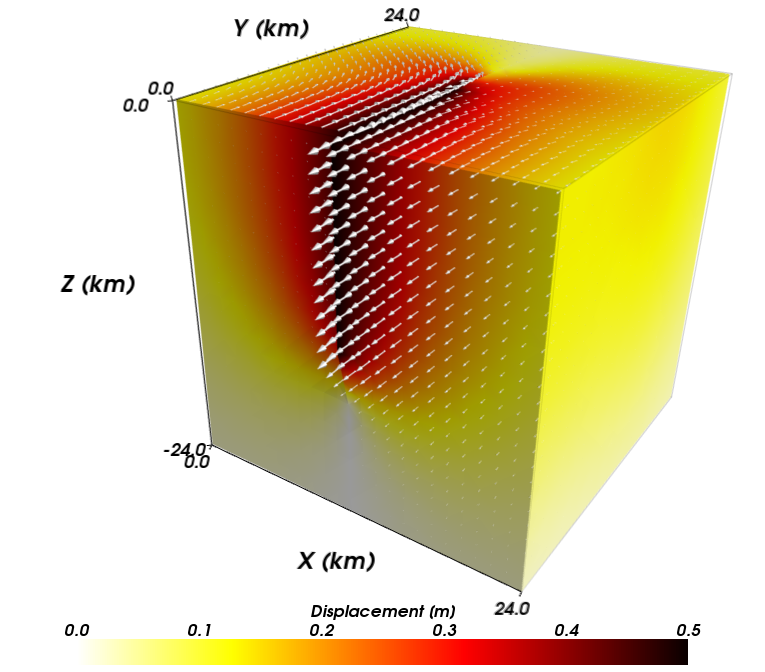
\includegraphics[scale=0.33]{benchmarks/strikeslip/figs/soln}
\par\end{centering}

\caption{Displacement field for strike-slip benchmark problem.\label{fig:benchmark:strikeslip:solution}}
\end{figure}



\subsubsection{Solution Accuracy}

We quantify the error in the finite-element solution by integrating
the L2 norm of the difference between the finite-element solution
 and the semi-analytical solution evaluated at the quadrature points.
We define the local error (error for each finite-element cell) to
be
\begin{equation}
\epsilon_{local}=\frac{1}{V_{cell}}\sqrt{\intop_{cell}\left(u_{i}^{t}-u_{i}^{fem}\right)^{2}\: dV},
\end{equation}
where $u_{i}^{t}$ is the ith component of the displacement field
for the semi-analytical  solution, and $u_{i}^{fem}$ is the ith component
of the displacement field for the finite-element  solution.  Taking
the square root of the L2 norm and normalizing by  the volume of the
cell results in an error metric with dimensions of length.  This roughly
corresponds to the error in the magnitude of the displacement field
in the finite element solution. We define the global error in a similar
fashion,
\begin{equation}
\epsilon_{global}=\frac{1}{V_{domain}}\sqrt{\intop_{domain}\left(u_{i}^{t}-u_{i}^{fem}\right)^{2}\: dV},
\end{equation}
 where we sum the L2 norm computed for the local error over all of
the  cells before taking the square root and dividing by the volume
of the domain. CIG has developed a package called Cigma \url{geodynamics.org/cig/software/packages/cs/cigma}
that computes these local and global error metrics.

Figures \ref{fig:benchmark:strikeslip:tet4:1000m} through \ref{fig:benchmark:strikeslip:hex8:250m}
show the local error for each of the three resolutions and two cell
types. The error decreases with decreasing cell size as expected for
a converging solution. The largest errors, which approach 1 mm for
1 m of slip for a discretization size of 250 m, occur where the gradient
in slip is discontinuous at the boundary between the region of uniform
slip and linear taper in slip. The linear basis functions cannot match
this higher order variation. The trilinear basis functions in the
hexahedral element provide more terms in the polynomial defining the
variation in the displacement field within each cell compared to the
linear basis functions for the tetrahedral cell. Consequently, for
this problem the error for the hexahedral cells at a given resolution
is smaller than that for the tetrahedral cells. Both sets of cell
types and basis functions provide the same rate of convergence as
shown in Figure \vref{fig:benchmark:strikeslip:convergence}.

\noindent \begin{center}
\begin{figure}[H]
\begin{centering}
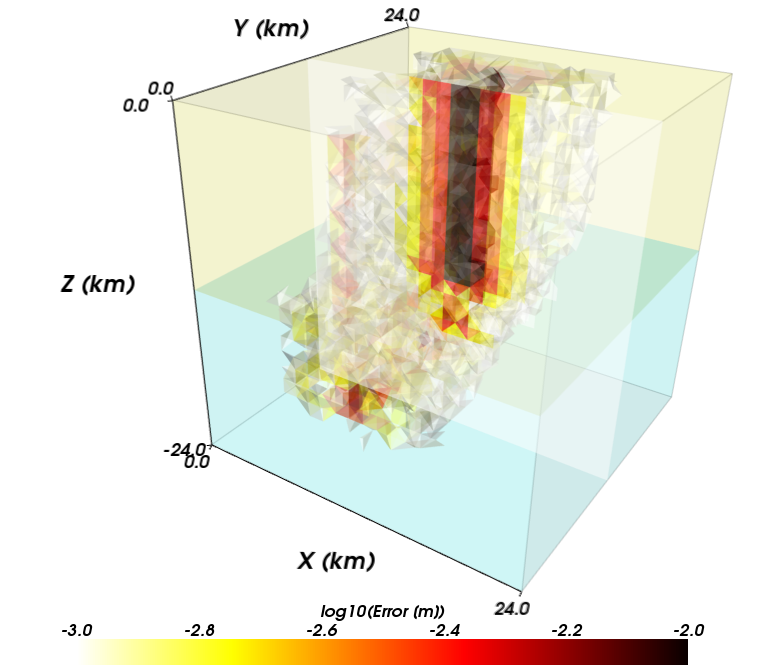
\includegraphics[scale=0.33]{benchmarks/strikeslip/figs/error_tet4_1000m}
\par\end{centering}

\caption{Local error for strike-slip benchmark problem with tetrahedral cells
and linear basis functions with a uniform discretization size of 1000
m.\label{fig:benchmark:strikeslip:tet4:1000m}}
\end{figure}

\par\end{center}

\noindent \begin{center}
\begin{figure}[H]
\begin{centering}
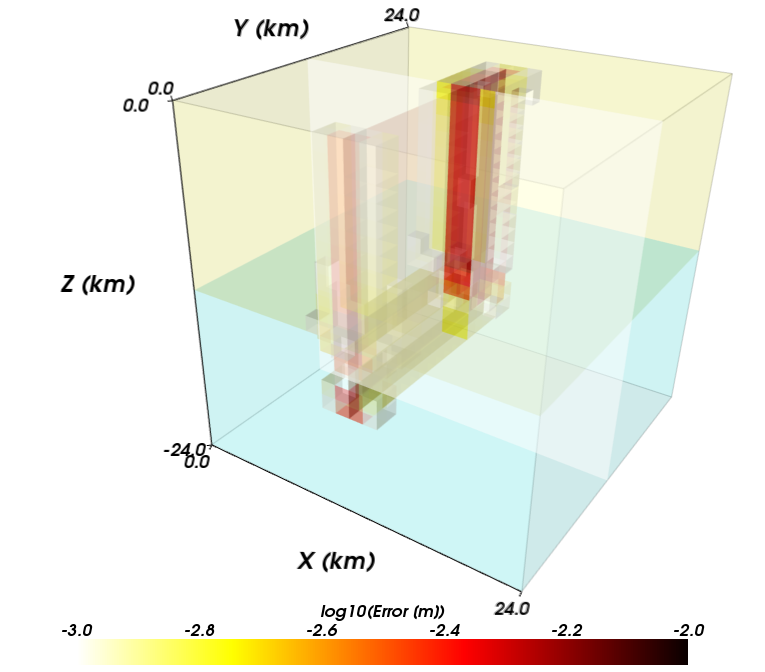
\includegraphics[scale=0.33]{benchmarks/strikeslip/figs/error_hex8_1000m}
\par\end{centering}

\caption{Local error for strike-slip benchmark problem with hexahedral cells
and trilinear basis functions with a uniform discretization size of
1000 m.\label{fig:benchmark:strikeslip:hex8:1000m}}
\end{figure}

\par\end{center}

\noindent \begin{center}
\begin{figure}[H]
\begin{centering}
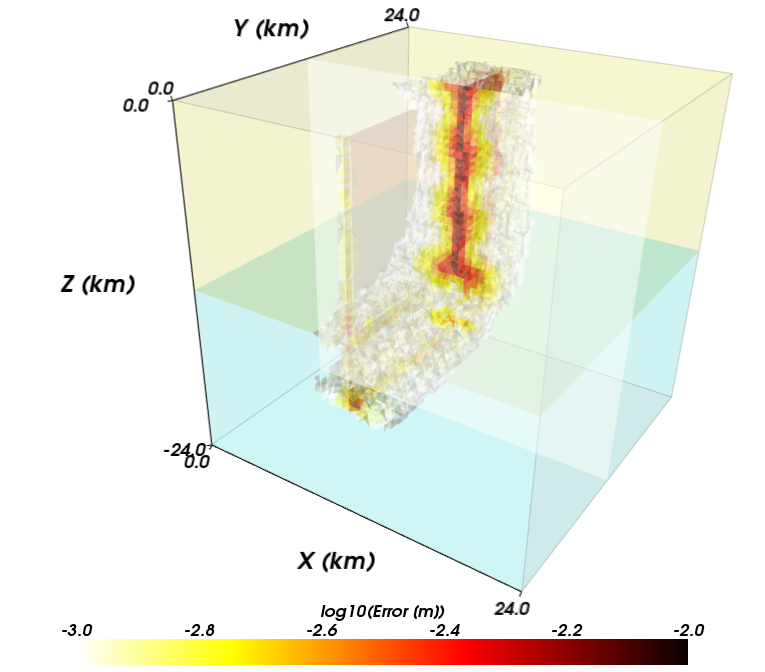
\includegraphics[scale=0.33]{benchmarks/strikeslip/figs/error_tet4_0500m}
\par\end{centering}

\caption{Local error for strike-slip benchmark problem with tetrahedral cells
and linear basis functions with a uniform discretization size of 500
m.\label{fig:benchmark:strikeslip:tet4:500m}}
\end{figure}

\par\end{center}

\noindent \begin{center}
\begin{figure}
\begin{centering}
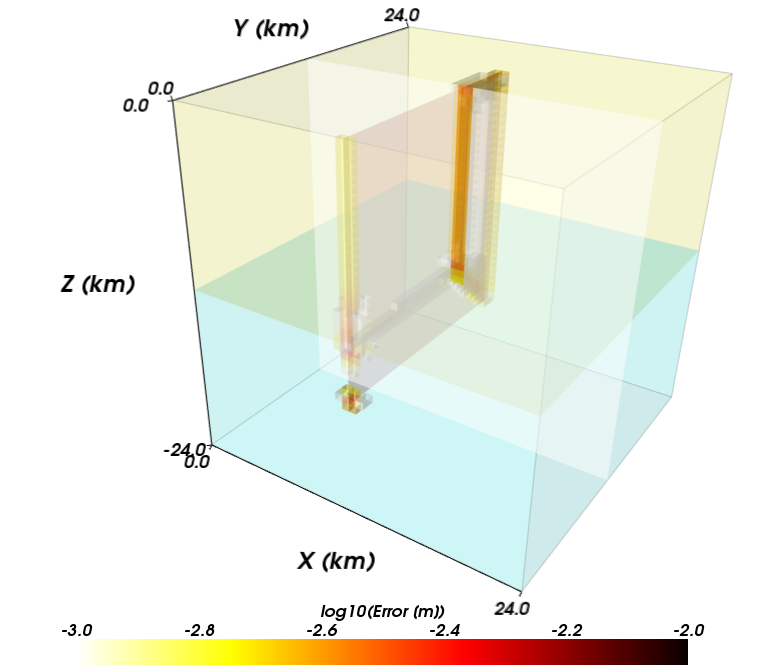
\includegraphics[scale=0.33]{benchmarks/strikeslip/figs/error_hex8_0500m}
\par\end{centering}

\caption{Local error for strike-slip benchmark problem with hexahedral cells
and trilinear basis functions with a uniform discretization size of
500 m.\label{fig:benchmark:strikeslip:hex8:500m}}
\end{figure}

\par\end{center}

\noindent \begin{center}
\begin{figure}[H]
\begin{centering}
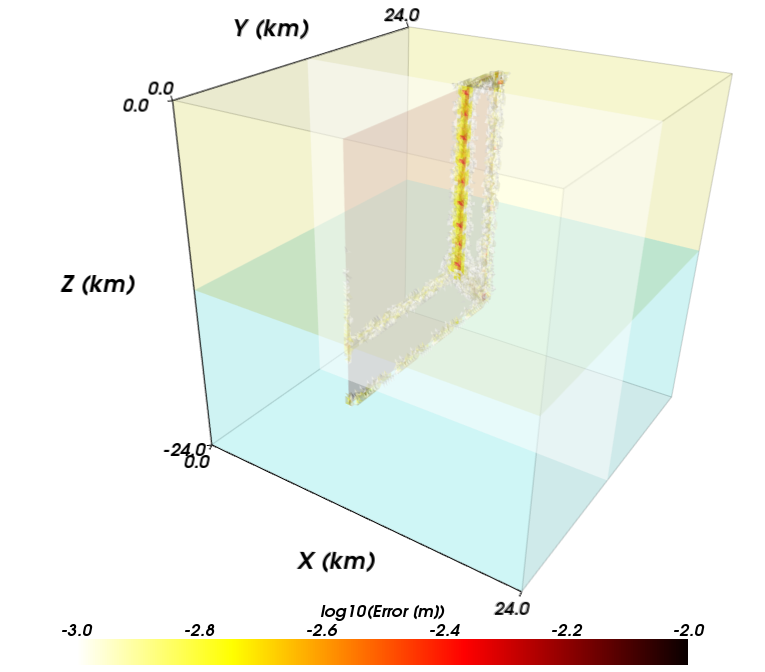
\includegraphics[scale=0.33]{benchmarks/strikeslip/figs/error_tet4_0250m}
\par\end{centering}

\caption{Local error for strike-slip benchmark problem with tetrahedral cells
and linear basis functions with a uniform discretization size of 250
m.\label{fig:benchmark:strikeslip:tet4:250m}}
\end{figure}

\par\end{center}

\noindent \begin{center}
\begin{figure}[H]
\begin{centering}
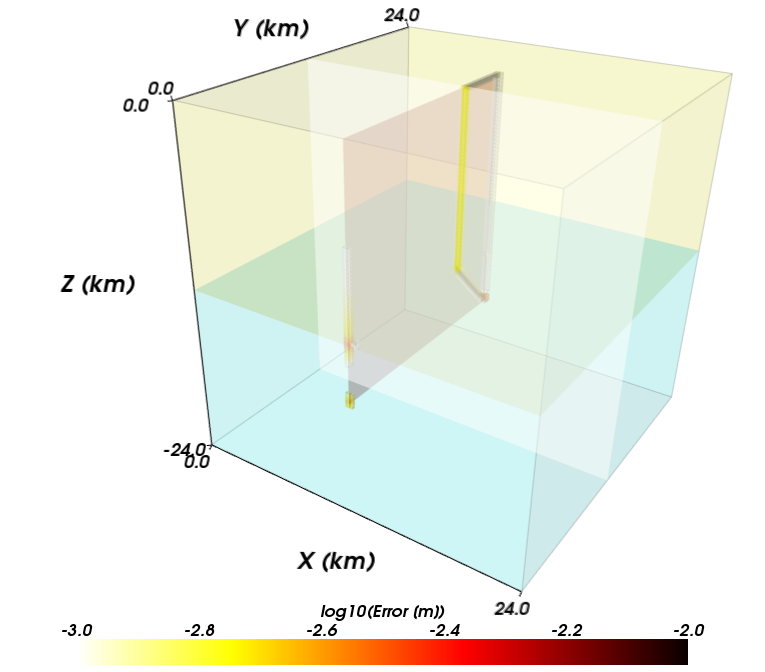
\includegraphics[scale=0.33]{benchmarks/strikeslip/figs/error_hex8_0250m}
\par\end{centering}

\caption{Local error for strike-slip benchmark problem with hexahedral cells
and trilinear basis functions with a uniform discretization size of
250 m.\label{fig:benchmark:strikeslip:hex8:250m}}
\end{figure}

\par\end{center}

\noindent \begin{center}
\begin{figure}[H]
\begin{centering}
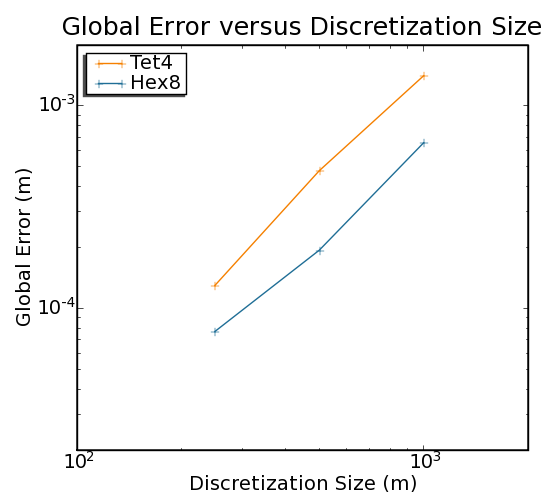
\includegraphics[scale=0.33]{benchmarks/strikeslip/figs/convergence}
\par\end{centering}

\caption{Convergence rate for the strike-slip benchmark problem with tetrahedral
cells and linear basis functions and with hexahedral cells with trilinear
basis functions.\label{fig:benchmark:strikeslip:convergence}}
\end{figure}

\par\end{center}


\subsubsection{Performance}

Figure \ref{fig:benchmark:strikeslip:summary} summarizes the overall
performance of each of the six simulations. Although at a given resolution,
the number of degrees of freedom in the hexahedral and tetrahedral
meshes are the same, the number of cells in the tetrahedral mesh is
about six times greater. However, we use only one integration point
per tetrahedral cell compared to eight for the hexahedral cell. This
leads to approximately the same number of integration points for the
two meshes, but the time required to unpack/pack information for each
cell from the finite-element data structure is greater than the time
required to do the calculation for each quadrature point (which can
take advantage of the very fast, small memory cache in the processor).
As a result, the runtime for the simulations with hexahedral cells
is significantly less than that for the tetrahedral cells at the same
resolution. 

\noindent \begin{center}
\begin{figure}[H]
\begin{centering}
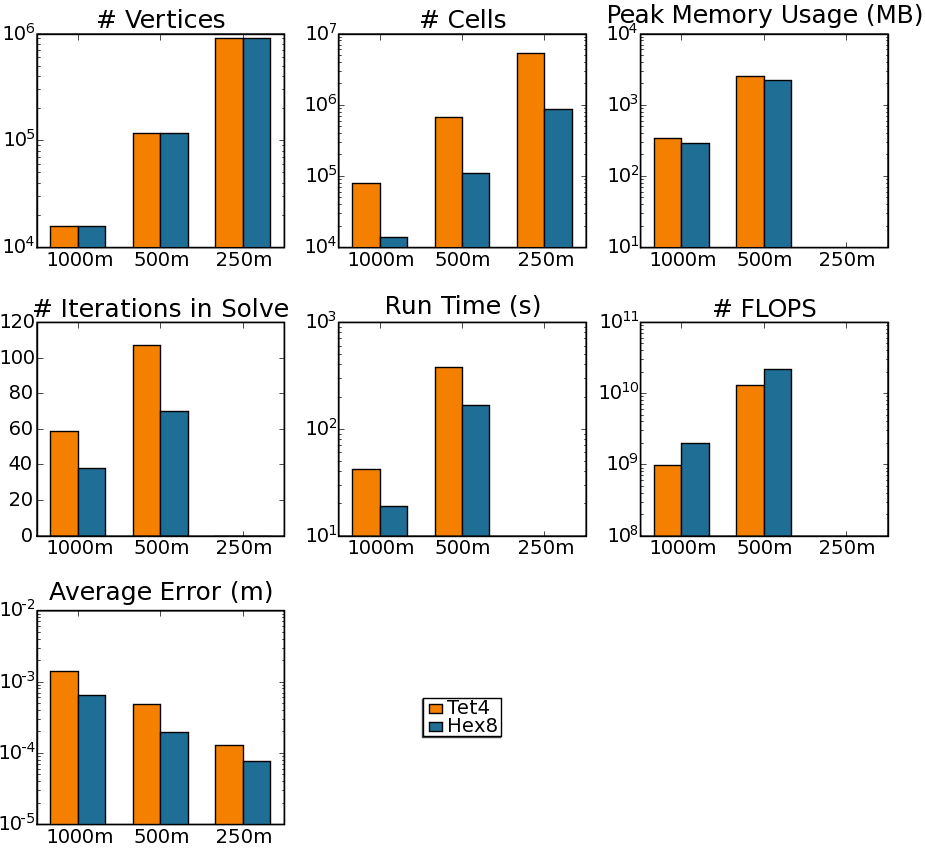
\includegraphics[scale=0.5]{benchmarks/strikeslip/figs/summary}
\par\end{centering}

\caption{Summary of performance of PyLith for the six simulations of the strike-slip
benchmark. For a given discretization size, hexahedral cells with
trilinear basis functions provide greater accuracy with a shorter
runtime compared with tetrahedral cells and linear basis functions.\label{fig:benchmark:strikeslip:summary}}
\end{figure}

\par\end{center}

Figure \vref{fig:benchmark:strikeslip:scaling} compares the runtime
for the benchmark (elastic solution only) at 500 m resolution for
1 to 16 processors. The total runtime is the time required for the
entire simulation, including initialization, distributing the mesh
over the processors, solving the problem in parallel, and writing
the output to VTK files. Some initialization steps, writing the output
to VTK files, and distributing the mesh are essentially serial processes.
For simulations with many time steps these steps will generally occupy
only a fraction of the runtime, and the runtime will be dominated
by the solution of the equations. Figure \ref{fig:benchmark:strikeslip:scaling}
also shows the total time required to form the Jacobian of the system,
form the residual, and solve the system. These steps provide a more
accurate representation of the parallel-performance of the computational
portion of the code and show excellent performance as evident in the
approximately linear slope of 0.7. S linear decrease with a slope
of 1 would indicate strong scaling, which is rarely achieved in real
applications.

\noindent \begin{center}
\begin{figure}[H]
\begin{centering}
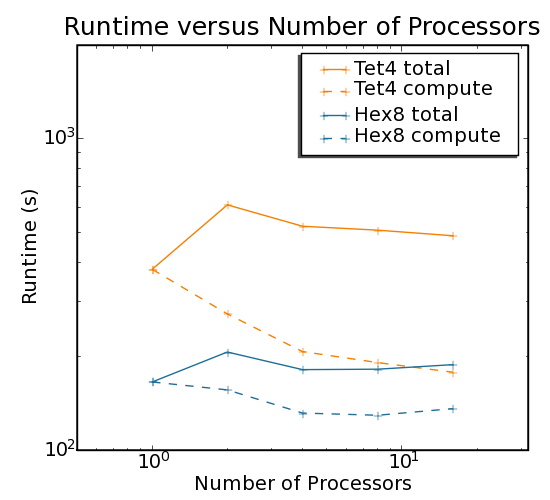
\includegraphics[scale=0.75]{benchmarks/strikeslip/figs/scaling}
\par\end{centering}

\caption{Parallel performance of PyLith for the strike-slip benchmark problem
with tetrahedral cells and linear basis functions with a uniform discretization
size of 500 m. The total runtime (total) and the runtime to compute
the Jacobian and residual and solve the system (compute) are shown.
The compute runtime decreases with a slope of about 0.7; a linear
decrease with a slope of 1 would indicate strong scaling,  which is
rarely achieved in any real application. \label{fig:benchmark:strikeslip:scaling}}
\end{figure}

\par\end{center}
\section{Savage and Prescott Benchmark}
\label{sec:benchmarks:savageprescott}

This benchmark problem computes the viscoelastic (Maxwell) relaxation
of stresses from repeated infinite, strike-slip earthquakes in 3D
without gravity. The files needed to run the benchmark may be found
at \url{https://github.com/geodynamics/pylith_benchmarks/tree/master/quasistatic/sceccrustdeform/savageprescott}.
An analytical solution to this problem is described by Savage and
Prescott \cite{Savage:Prescott:1978}, which provides a simple way
to check our numerical solution. A python utility code is provided
in the utils directory to compute the analytical solution. Although
this problem is actually 2.5D (infinite along-strike), we solve it
using a 3D finite element model.


\subsection{Problem Description}

Figure \ref{fig:benchmark:savageprescott:geometry} shows the geometry
of the problem, as described by \cite{Savage:Prescott:1978}. The
analytical solution describes the surface deformation due to repeated
earthquakes on an infinite strike-slip fault embedded in an elastic
layer overlying a Maxwell viscoelastic half-space. The upper portion
of the fault (red in the figure) is locked between earthquakes, while
the lower portion (blue in the figure) creeps at plate velocity. At
regular recurrence intervals, the upper portion of the fault abruptly
slips by an amount equal to the plate velocity multiplied by the recurrence
interval, thus 'catching up' with the lower part of the fault.

There are some differences between the analytical solution and our
numerical representation. First, the analytical solution represents
the earthquake cycle as the superposition of uniform fault creep and
an elementary earthquake cycle. Uniform fault creep is simply the
uniform movement of the two plates past each other at plate velocity.
For the elementary earthquake cycle, no slip occurs below the locked
portion of the fault (blue portion in the figure). On the locked (red)
portion of the fault, backslip equal to plate velocity occurs until
the earthquake recurrence interval, at which point abrupt forward
slip occurs. In the finite element solution, we perform the simulation
as described in the figure. Velocity boundary conditions are applied
at the extreme edges of the model to simulate block motion, steady
creep is applied along the blue portion of the fault, and regular
earthquakes are applied along the upper portion of the fault. It takes
several earthquake cycles for the velocity boundary conditions to
approximate the steady flow due to steady block motion, so we would
not expect the analytical and numerical solutions to match until several
earthquakes have occurred. Another difference lies in the dimensions
of the domain. The analytical solution assumes an infinite strike-slip
fault in an elastic layer overlying a Maxwell viscoelastic half-space.
In our finite element model we are restricted to finite dimensions.
We therefore extend the outer boundaries far enough from the region
of interest to approximate boundaries at infinity.

Due to the difficulties in representing solutions in an infinite domain,
there are several meshes that have been tested for this problem. The
simplest meshes have uniform resolution (all cells have equal dimensions);
however, such meshes typically do not provide accurate solutions since
the resolution is too coarse in the region of interest. For that reason,
we also tested meshes where the mesh resolution decreases away from
the center. In the problem description that follows, we will focus
on the hexahedral mesh with finer discretization near the fault
({\tt meshes/hex8\_6.7km.exo.gz}), which provides a good match
with the analytical solution. It will first be necessary to gunzip
this mesh so that it may be used by PyLith.
\begin{description}
\item [Domain] The domain for this mesh spans the region
\begin{gather*}
-1000\leq x\leq1000\ km,\\
-500\leq y\leq500\ km,\\
-400\ km\leq z\leq0.
\end{gather*}
The top (elastic) layer occupies the region $-40\ km\ \leq z\leq0$
and the bottom (viscoelastic) layer occupies the region $-400\ km\ \leq z\leq-40\ km$.
\item [Material~properties] The material is a Poisson solid with a shear
modulus ($\mu$) of 30 GPa. The domain is modeled using an elastic
isotropic material for the top layer and a Maxwell viscoelastic material
for the bottom layer. The bottom layer has a viscosity ($\eta$) of
2.36682e+19 Pa-s, yielding a relaxation time ($2\eta/\mu$) of 50
years.
\item [Fault] The fault is a vertical, left-lateral strike-slip fault.
The strike is parallel to the y-direction at the center of the model:
\begin{gather*}
x=0\ km,\\
-500\leq y\leq500\ km,\\
-40\ km\leq z\leq0.
\end{gather*}
The locked portion of the fault (red section in Figure \ref{fig:benchmark:savageprescott:geometry})
extends from $-20\: km\leq z\leq0$, while the creeping section (blue)
extends from $-40\: km\leq z\leq0$. Along the line where the two
sections coincide ($z=-20\: km$), half of the coseismic displacement
and half of the steady creep is applied (see \texttt{finalslip.spatialdb}
and \texttt{creeprate.spatialdb}).
\item [Boundary~conditions] On the bottom boundary, vertical displacements
are set to zero, while on the y-boundaries the x-displacements are
set to zero. On the x-boundaries, the x-displacements are set to zero,
while constant velocities of +/- 1 cm/yr are applied in the y-direction,
giving a relative plate motion of 2 cm/year.
\item [Discretization] For the nonuniform hexahedral mesh, the resolution
at the outer boundaries is 20 km. An inner region is then put through
one level of refinement, so that near the center of the mesh the resolution
is 6.7 km. All meshes were generated with CUBIT.
\item [Basis~functions] We use trilinear hexahedral cells.
\item [Solution] We compute the surface displacements and compare these
to the analytical solution in Figure \ref{fig:benchmark:savageprescott:solution}.
\end{description}

\begin{figure}[htbp]
  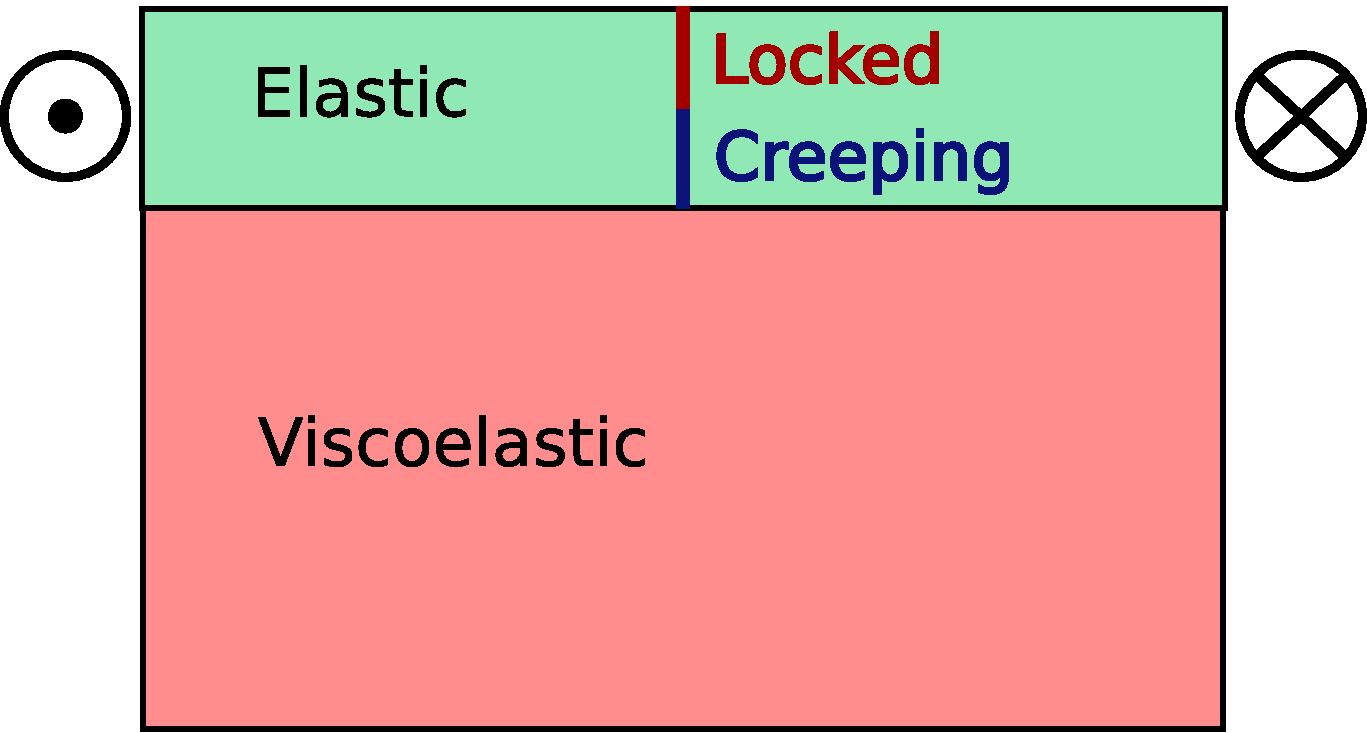
\includegraphics[scale=0.33]{benchmarks/figs/savageprescott_diagram}
  \caption{Problem description for the Savage and Prescott strike-slip
    benchmark problem.}
  \label{fig:benchmark:savageprescott:geometry}
\end{figure}


\subsection{Running the Benchmark}

There are a number of {\tt .cfg} files corresponding to the
different meshes, as well as a {\tt pylithapp.cfg} file defining
parameters common to all problems. Each problem uses four
{\tt .cfg} files: {\tt pylithapp.cfg}, {\tt fieldsplit.cfg}
(algrebraic multigrid preconditioner), a cell-specific file (e.g.,
{\tt hex8.cfg}), and a resolution specific file (e.g.,
hex8\_6.7km.cfg).

\begin{shell}
# If you have not do so already, checkout the benchmarks from the CIG Git repository.
$ git clone https://github.com/geodynamics/pylith_benchmarks.git
# Change to the quasistatic/sceccrustdeform/savageprescott directory.
$ cd quasistatic/sceccrustdeform/savageprescott
# Decompress the gzipped files in the meshes directory.
$ gunzip meshes/*.gz
# Run one of the simulations.
$ pylith hex8.cfg hex8_6.7km.cfg fieldsplit.cfg
\end{shell}

Each simulation uses 10 earthquake cycles of 200 years each,
using a time-step size of 10 years, for a total simulation time of
2000 years. Ground surface output occurs every 10 years, while all
other outputs occur every 50 years.

Once the problem has run, results will be placed in the {\tt output}
directory. These results may be viewed directly using 3-D
visualization software such as ParaView; however, to compare results
to the analytical solution, some postprocessing is required. First,
generate the analytical results by running the {\tt calc\_analytic.py}
script. This will produce files with displacements and velocities
({\tt analytic\_disp.txt} and {\tt analytic\_vel.txt}) in the {\tt
  output} directory that are easy to use with a plotting package, such
as matplotlib or Matlab.


\subsection{Benchmark Results}

Figure \ref{fig:benchmark:savageprescott:solution} shows the computed
surface displacements for the 10th earthquake cycle compared with
the analytical solution. The profile results were obtained as described
above, and then all results (analytical and numerical) were referenced
to the displacements immediately following the last earthquake. We
find very good agreement between the analytical and numerical solutions,
even for meshes with uniform refinement. We have not yet explored
quantitative fits as a function of mesh resolution. For this benchmark,
it is also important to consider the distance of the boundary from
the region of interest. Also note that the agreement between analytical
and numerical solutions is poor for early earthquake cycles, due to
the differences in simulating the problem, as noted above.

\begin{figure}[htbp]
  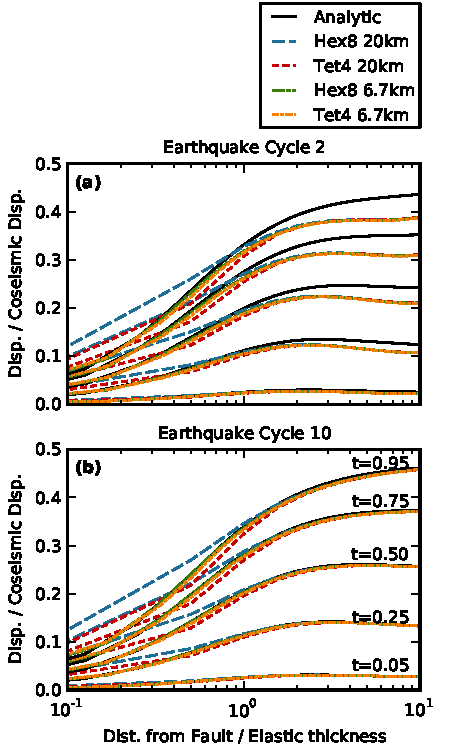
\includegraphics[scale=0.66]{benchmarks/figs/savageprescott_soln_profiles}
  \caption{Displacement profiles perpendicular to the fault for a
    PyLith simulation with hex8 cells and the analytical solution for
    earthquake cycle 10.}
  \label{fig:benchmark:savageprescott:solution}
\end{figure}

% End of file



\section{SCEC Dynamic Rupture Benchmarks}

The SCEC website \url{scecdata.usc.edu/cvws/cgi-bin/cvws.cgi} includes
a graphical user interface for examining the benchmark results. Benchmark
results for PyLith are available for TPV205-2D (horizontal slice through
a vertical strike-slip fault), TPV205 (vertical strike-slip fault
with high and low stress asperities), TPV210-2D (vertical slice through
a 60-degree dipping normal fault), TPV210 (60-degree dipping normal
fault), TPV11, TPV12, TPV13, TPV14-2D and TPV15-2D (horizontal slice
through a verticel strike-slip fault with a branch), TPV14, TPV15,
TPV 24, TPV25 (vertical strike-slip fault with a branch), TPV 16 and
17 (vertical strike-slip fault with spatially heterogeneous initial
tractions), TPV 22 and 23 (vertical strike-slip fault with a stepover),
TPV102 (vertical strike-slip fault with rate-state friction).

The benchmark results indicate that triangular and tetrahedral cells
generate less numerical noise than quadrilateral or hexahedral cells.
The input files in the repository are updated for PyLith v2.0.0, so
you will need to modify them if you use another version of PyLith.
